\chapter{Mathematical Background}

Multi-agent systems are frequently modeled as a distributed optimization problem. The optimization problem has to search for an optimal solution taking into account a big number of local and neighbor constraints. Indeed, it is important to implement strategies to communicate and control in a coordinated way the interconnect network. This chapter presents an overview of the different techniques used for this purpose. Some of them are related to model and analyze the network of agents, while others are related to control and search for an optimal solution to an optimization problem. The chapter begins with a small introduction to graph theory and continues with different optimization theories. 

\section{Graph Theory}


\begin{figure}[h]
\begin{center}
    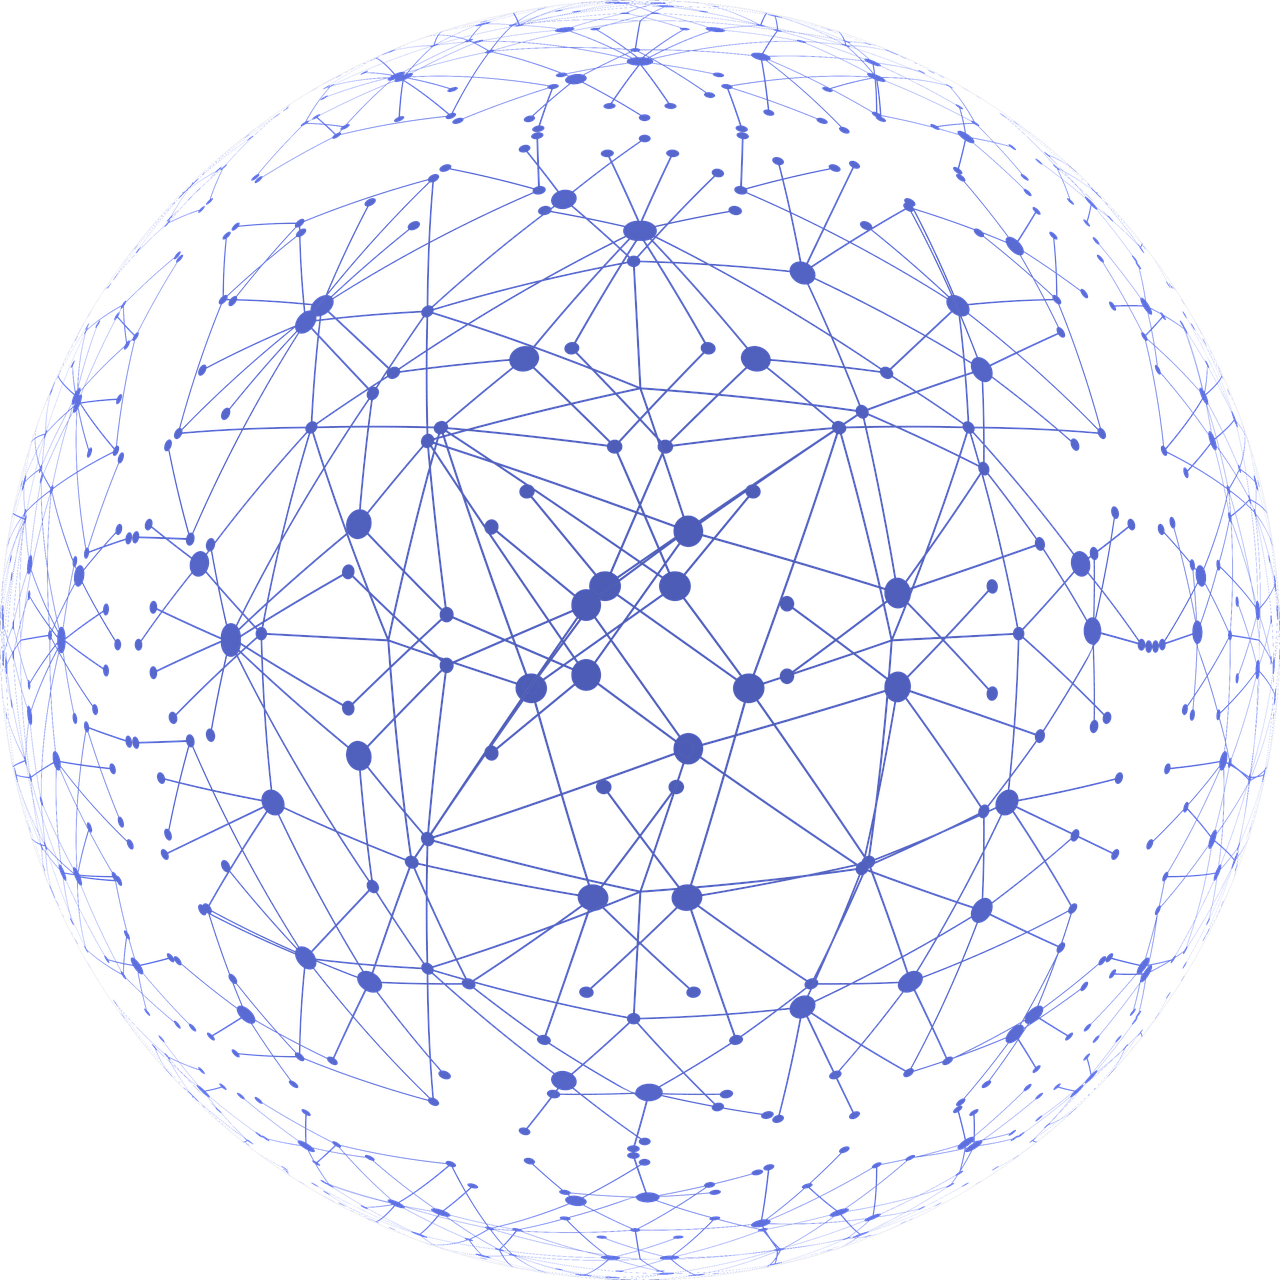
\includegraphics[width=0.3\textwidth]{Kap2/Network.png}
    \caption{Social Network.}
    \label{Social_net}
\end{center}
\end{figure}

In an interconnected system, it is important to model the entire system allowing it to apply analysis and control techniques. A common way to represent a set of interconnected agents is a graph (Fig. \ref{Social_net}). It is a representation of the connections, weights, nodes, and structure of the network. The Graph is as a set of finite elements composed of nodes $\mathcal{V}$ and edges $\mathcal{E}$ . The set of  nodes $\mathcal{V}$ represent each agent, and it has the form $\mathcal{V} =  \left \{ v_{1},v_{2},...,v_{n} \right \}$ and its connections or edges has the form $\mathcal{E} =  \left \{ v_{1}v_{2},v_{2}v_{3},...,v_{i}v_{j} \right \}$. A finite graph is built by join its edges and nodes, see Fig. \ref{Graph}. This union is defined as: 


\begin{equation}
 \mathcal{G}=(\mathcal{V},\mathcal{E})   
\end{equation}
The neighborhood of node $v_{i}$ is the set of nodes $\mathcal{N}_{i} \subseteq  \mathcal{V}$ that have a direct interaction with agent $i$. This set of edges could be directed or undirected depending on the way of communication between them. A graph $\mathcal{G}$ is connected if a connection exists between two or more nodes and there is a route between all nodes in the set $\mathcal{V}$. Lastly, the set of nodes of a graph has a degree that depends on the number of neighbors of each node. If all nodes of a graph have the same degree, the graph is called a regular graph.

A graph could be represented as a joint of multiple matrices. These matrices show information about each node with the other. 



\begin{figure}[h]
\begin{center}
    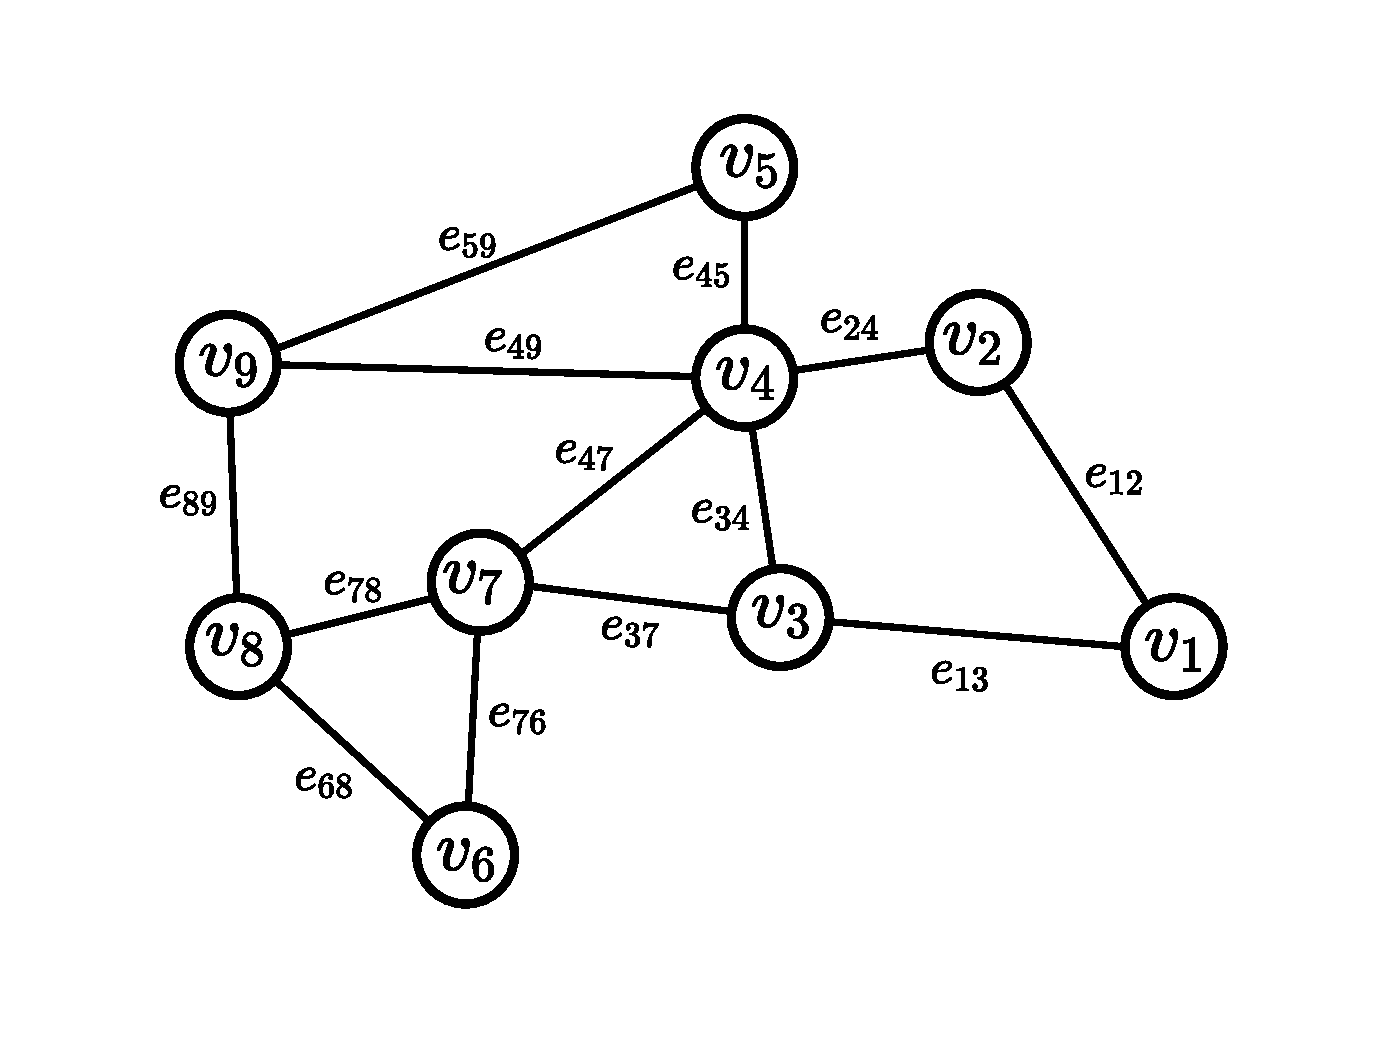
\includegraphics[width=0.7\textwidth]{Kap2/Graph-01.eps}
    \caption{ Graph of Network system.}
    \label{Graph}
\end{center}
\end{figure}



\section*{Degree and Adjacency Matrix}

The degree of a node $v_{i}$ is represented as $d(v_{i})$, which is the name of the cardinality of a node and it represents the number of agents connected with node $i$. Therefore, The degree matrix is a diagonal matrix with the degree values of each node:

\begin{equation}
    \Delta (\mathcal{G}) = \begin{bmatrix}
d(v_{1}) &   0    &  \cdots & 0\\ 
0      & d(v_{2}) & \cdots &  0 \\ 
\vdots & \vdots   & \ddots  & \vdots\\ 
0      & 0        & \cdots & d(v_{n}) 
  \end{bmatrix}
\end{equation}

In addition, an adjacency matrix exists where the relationship of each node with each other is represented. Moreover, the adjacency matrix is defined as:

\begin{equation}
    \left [ Y(\mathcal{G}) \right ]_{ij} = \left\{\begin{matrix}
1, & \text{if } v_{i}v_{j} \in \mathcal{E},\\ 
0, & \text{Otherwise.} 
\end{matrix}\right.
\end{equation}

\section*{Incidence Matrix}
There exist direction or bi-direction graphs in its edges. If a graph exists with directed edges, it is called a digraph $\mathcal{D}$. Therefore, a digraph is described in its incidence matrix, where it is a representation of the orientation of each edge of the graph. This information is useful to evaluate network stability and controllability. This representation is defined as:

\begin{equation}
    I_{ij}(\mathcal{G}) = \left\{\begin{matrix*}[l]
-1, & \text{if } v_{i} \text{ is the tail of } v_{j},\\ 
1, & \text{if } v_{i} \text{ is the head of } v_{j},\\ 
0, &  \text{Otherwise.   }
\end{matrix*}\right.
\end{equation}

A graph could also have weights in its connections, which represent the amount of influence of neighbors on each node. If a graph has weighted edges, it is called a weight graph. Consequently, in a weight graph the adjacency matrix is built by the next definition:


\begin{equation}
    Ad(\mathcal{G}) = \left\{\begin{matrix}
\omega_{ij},   & \text{if } (v_{i}v_{j}) \in \mathcal{E}, \\ 
0, &  \text{Otherwise.}
\end{matrix}\right.
\end{equation}


\section*{Laplacian}

The Laplacian of a graph is another fundamental representation of a graph. The way of representing a Laplacian graph of a graph $\mathcal{G}$ is by using the joint of adjacency and degree matrix as follows:

\begin{equation}
    L(\mathcal{G}) = \Delta (\mathcal{G}) - Y\mathcal(G)
\end{equation}

Laplacian matrix must be symmetric if it is a digraph, or asymmetric otherwise. 










% representacion matricial de grafos

% matriz de grafo y de adyacencia 






\section{Model Predictive Control}

Model Predictive Control (MPC) is an advanced control method used to control a set of variables that satisfy a group of constraints. MPC is based on the optimization of a finite horizon prediction of a system model. The principal idea is to predict and optimize future decisions in a specific future time, satisfying a model of the entire system and some constraints. This section describes the mathematical theory of a Model Predictive Control and its applications in the described system.



\begin{center}
    x(t+1) = f(x(t),u(t)),\label{eq:mpc2}\\
    y(t) = g(x(t),u(t)). \label{eq:mpc}
\end{center}



\subsection{Dynamic Prediction Model}

\subsection{Objective Function}

\subsection{Constraints}



\section{Alternate Direction Method of Multipliers}
% //////////// GAME THEORY ////////////
\section{Game Theory}
Game theory is defined in \cite{GameTheory2} as ``The study of mathematical models of conflict and cooperation between intelligent rational decision-makers". One way to see the control game theory is in competitive games, more commonly known as zero-sum games. There are 2 or more players trying to get the most benefit possible, but the benefit of one is the detriment of the other ones. Another way to see game theory in control theory is a conflict perspective. In a conflict perspective, the environment is a player and the controller is the other player. The main motivation of game theory is to achieve maximum profit for all players to getting close or achieving the goal. 
Also, game theory could be implemented in cooperative perspective. In cooperative way, there can be many agents with same objective function. The difficult is that different agents could have access to information about their neighbors. This information access difficult a centralized controller implementation. 
Another setting, 





\subsection{Potential Games}


